\chapter{Methodology}
In this chapter, the technical details of our methodology are described. We describe in \refsec{data-collection} the process of collecting the dataset; in \refsec{switchlm} the technique of our learned editing operations is elaborated; in \refsec{genco} the details of the contrastive learning framework are presented.

\section{\texttt{MultiAgencyNews} Data Collection}
\label{data-collection}
The data collection has two main phases:
\begin{enumerate}
    \item Web scraping structured article metadata from \texttt{ground.news}
    \item Collecting the full news article information from news agency websites.
\end{enumerate}
We provide background information of \texttt{ground.news} in \refsec{ground-news}, details on these two phases in \refsec{article-metadata} and \refsec{full-news}, and statistics in \refsec{dataset-stats}.

\subsection{\texttt{Ground.news} Background Information}
\label{ground-news}
\texttt{Ground.news} is a News Aggregation platform, where news articles from different news agencies are aggregated and presented together. \texttt{Ground.news} has a \textit{topic-story-article} hierarchy, a screenshot of which is shown in \reffig{fig:ground-news}. There are three levels in the hierarchy, namely:
\begin{enumerate}
    \item \textit{Topic} is the highest level, which can be one of the following four kinds:
    \begin{enumerate}
        \item abstract topics such as ``politics'' or ``trade'';
        \item geopolitical concepts such as ``iran'' or ``pakistan'';
        \item specific celebrities, such as ``tim-cook'' or ``liz-truss'';
        \item news sources, such as npr or new-york-times.
    \end{enumerate}
    \item \textit{Story} is the middle level, which is an event that got coverage from different sources. \Eg, ``elon-musk-and-twitter-discussed-price-cut-to-44-billion-takeover-in-recent-weeks'' contains news articles covering the recent event that concerns the recently acquisition by Elon Musk.
    \item \textit{Article} is the lowest level, which contains the metadata of an article.
\end{enumerate}
\begin{figure}[ht!]
    \centering
    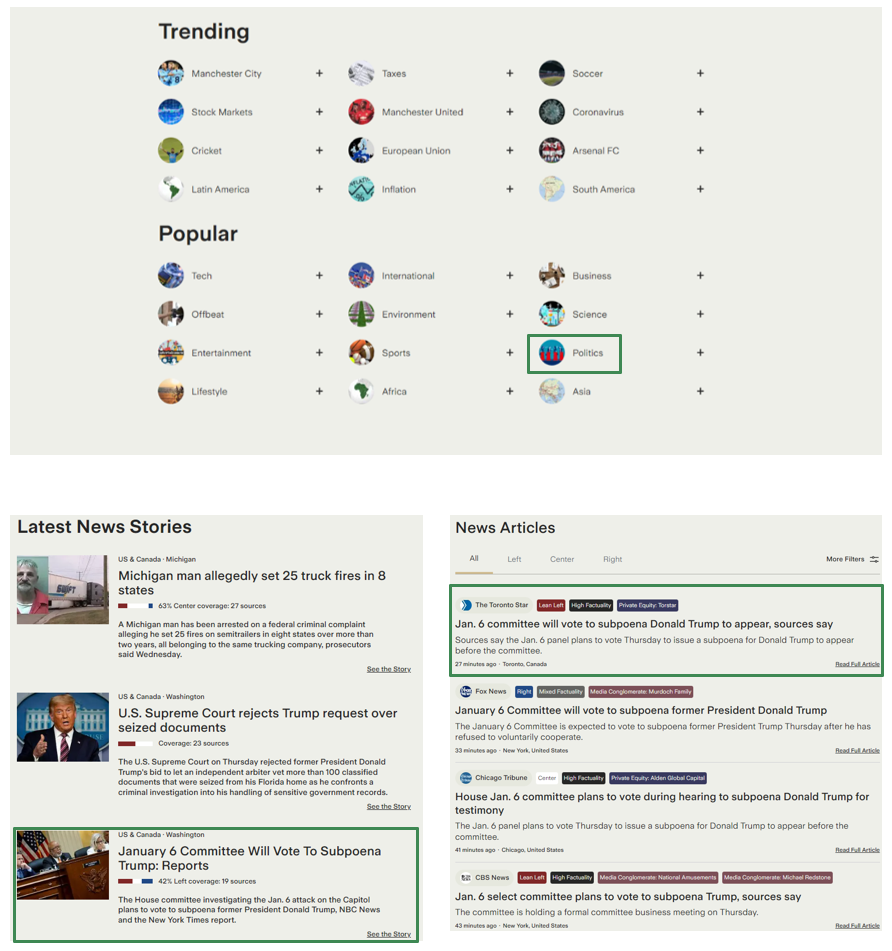
\includegraphics[width=0.95\textwidth]{img/ground_news.png}
    \caption{A Screeshot of \texttt{ground.news} (https://ground.news). The top figure displays a non-exhaustive list of the topics covered. The left bottom figure displays a list of \textit{stories} under the topic \textit{Politics}. The right bottom figure displays a list of news \textit{articles} from different news agencies for the \textit{story} ``January 6 committee ... Reports'', where metadata is provided.}
    \label{fig:ground-news}
\end{figure}

\subsection{Article Metadata}
\label{article-metadata}
To collect the news data, we need to first obtain the article metadata. We create a web scrapper\footnote{\url{https://github.com/liamjxu/ground\_news\_webscraper}} to collect article metadata from \texttt{ground.news}. The web scraper is based on the HTML parsing toolkit \texttt{BeautifulSoup} and the frontend testing toolkit \texttt{Selenium}. The web scraper starts with the root level of the topic list\footnote{\url{https://ground.news/my/discover}}. By mimicking the mouse-clicking events with \texttt{Selenium}, the sub-page of each topic is displayed. The web scrapper further parses the related section of the current topic web page to obtain more topics. This process can be modeled as a multi-source Breadth-First-Search process.

Then the story pages on each topic page are collected, which are then used to find metadata for each specific article. 
Among the metadata provided by \texttt{ground.news}, three kinds of metadata serve our purposes most substantially:
\begin{enumerate}
    \item \textit{bias} is the political stance category of the current news agency labeled by \texttt{ground.news} (one of ``Left'', ``Lean Left'', ``Center'', ``Lean Right'', ``Right'', ``Unknown'')
    \item \textit{factuality} is the news reliability category of the current news agency labeled by \texttt{ground.news} (one of ``High Factuality'', ``Low Factuality'', ``Mixed Factuality'', ``Unknown'')
    \item \textit{URL} is the link to the original news web page.
\end{enumerate}

Note that the original full text is not directly available to us. Thus, the \textit{URL} obtained in \refsec{article-metadata} is further processed in \refsec{full-news} to obtain the full information of the news articles.


\subsection{Full News Information Collection}
\label{full-news}
We utilized the \texttt{news-please} toolkit\footnote{\url{https://github.com/fhamborg/news-please}} to extract the news content information from the \textit{URL} provided by \texttt{ground.news} in \refsec{ground-news}. Namely, we collected the following attributes of the news articles:
\begin{enumerate}
    \item \textit{article\_idx}: the index of the article within the story;
    \item \textit{name}: name of the news agency;
    \item \textit{date\_publish}: the date the article got published;
    \item \textit{image\_url}: the URL to the news image (if any);
    \item \textit{language}: the language of the article;
    \item \textit{url}: the URL to the original article;
    \item \textit{source\_domain}: the source domain of the original article;
    \item \textit{title}: the article title;
    % \item \textit{authors}: the article author list;
    \item \textit{maintext}: the main text of the article.
\end{enumerate}

\subsection{Dataset Statistics}
\label{dataset-stats}
When the data collection is finished, the final dataset has the following statistics shown in \reftab{tab:dataset-stat}. The dataset is open-sourced \footnote{\url{https://github.com/blender-nlp/MultiAgencyNews}}.
\begin{table}[h]
    \centering
    \resizebox{0.5\columnwidth}{!}{%
    \begin{tabular}{@{}cc@{}}
    \toprule
    \textbf{Metric}              & \textbf{Number} \\ \midrule
    collected   topics           & 544             \\
    collected   stories          & 17,716          \\
    collected   articles         & 187,479         \\
    unique   urls                & 107,721         \\
    words in the unique articles & 54,631,854      \\ \bottomrule
    \end{tabular}%
    }
    \caption{The Statistics of the Collected Dataset}
    \label{tab:dataset-stat}
\end{table}


\section{\texttt{SwitchLM} Functionality Suites}
\label{switchlm}
We propose to conduct framing analysis on the \texttt{MultiAgencyNews} dataset. Specifically, we aim to answer the following questions:
\begin{quote}
    \textit{How to determine the underlying stance for news articles?} \\
    \textit{How to generate text with pre-set stance?}
\end{quote}
Correspondingly, we propose the \texttt{SwitchLM} Functionality Suites, which consist of the following two functionalities:
\begin{enumerate}
    \item Stance categorization upon given input text.
    \item Text generation controlled by input stance;
\end{enumerate}
In \refsec{switch-motivation}, we elaborate our motivation behind this design. We further provide the design details in \refsec{switch-model} and implementation details in \refsec{switch-implement}.

\subsection{Motivation}
\label{switch-motivation}
Different audiences with ranged stances can have varied perceptions of the same concept (\eg, guns), however, within the fixed vocabulary of generative language models, the word embedding for the same word is static across stances. This counter-intuitive setting motivated us to design means of adding another degree of freedom to allow cross-stance dynamic embedding.

Inspired by the steerability demonstrated in visual deep generative models, we hypothesized that a linear subspace in the word embedding space exists for natural language generation models, where the latent embeddings corresponding to stance-shifting operations align, as shown in \reffig{fig:switch-lm}. 
\begin{figure}[h]
    \centering
    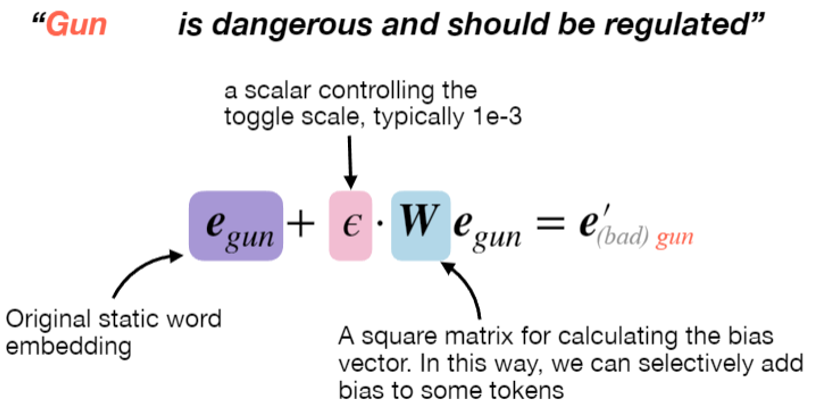
\includegraphics[width=0.8\textwidth]{img/switchLM.png}
    \caption{Learning a projection matrix for switching generative language models allows selective addition of stance shifts. }
    \label{fig:switch-lm}
\end{figure}

Here, $e$ is the original static word embedding from the pre-trained generative language model, and $e'$ is the stance-navigated word embedding. The projection matrix $W$ maps the embedding of each word in the vocabulary into a basis of their specific editing subspace. The scalar $\epsilon$ then controls the scale of stance shifting.

This hypothesis allows us to achieve the two functionalities as proposed in \refsec{switchlm}, as elaborated in \refsec{switch-model}.

\subsection{Model Design}
\label{switch-model}
We now describe our model design and explain how the functionalities in \refsec{switch-model} can be unified under the hypothesis in \refsec{switch-motivation} via this model design.

The high-level model architecture is shown in \reffig{fig:switch-design}. The linearly transformed word embeddings are only applied to the output layer of the generative models as a replacement for the original output embedding, and $W$ is the only learnable parameter in our model, which guarantees the parameter efficiency of the method.

\begin{figure}[ht]
    \centering
    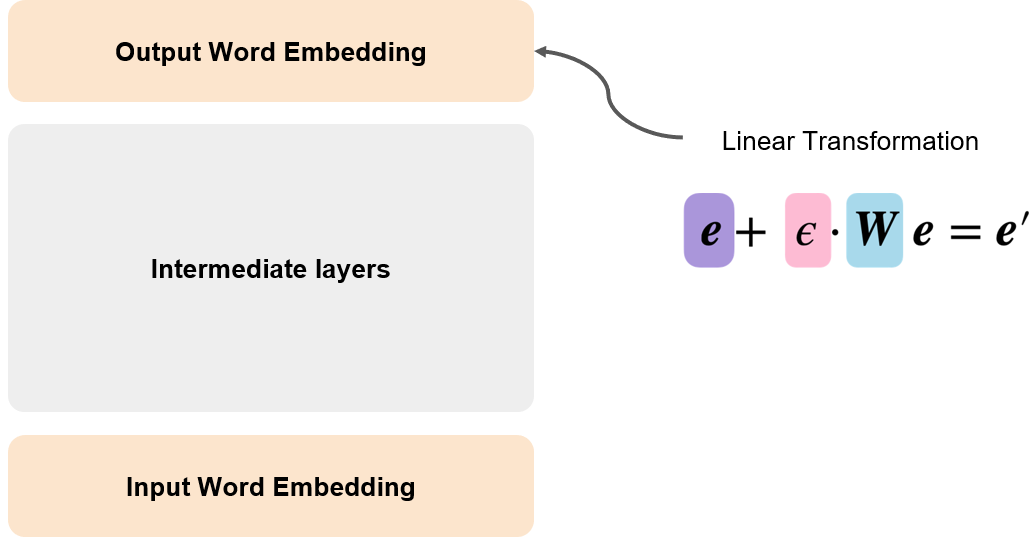
\includegraphics[width=\textwidth]{img/switch-design}
    \caption{The Model Architecture of \texttt{SwitchLM}.}
    \label{fig:switch-design}
\end{figure}

Corresponding to the two functionalities in \refsec{switchlm}, the model has two modes of application, shown in \reffig{fig:switch-func}. Under mode (a), the model conducts generation with a specified $\epsilon$ translated from the user input on a political stance spectrum. Under mode (b), the model operates under a frozen $W$ and profiles the probability of generating the given input with different $\epsilon$ and treats that distribution as the stance likelihood distribution. In this way, the model serves both the stance-guided generation functionality and the stance detection functionality.

\begin{figure}[h]
    \centering
    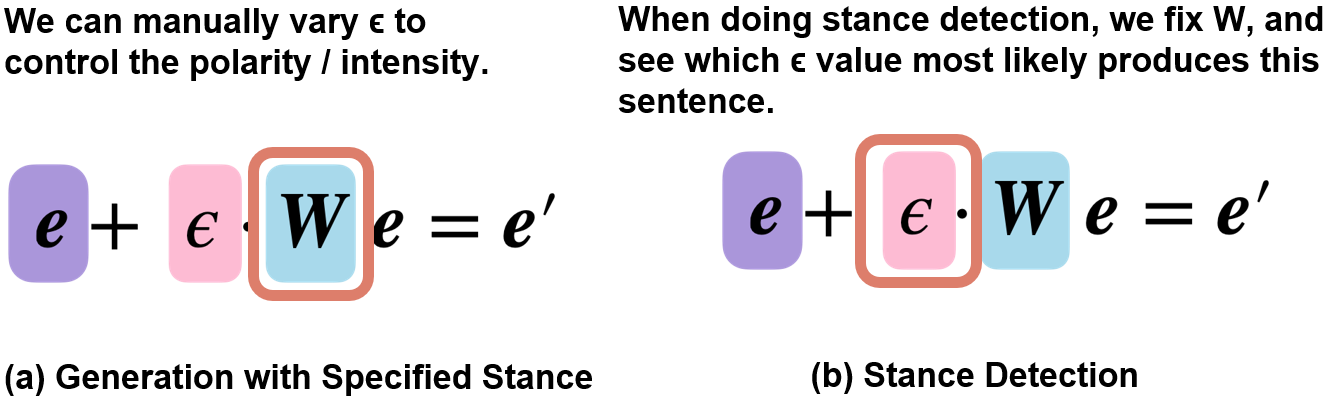
\includegraphics[width=\textwidth]{img/switch-func}
    \caption{The Two Modes of \texttt{SwitchLM}.}
    \label{fig:switch-func}
\end{figure}

\subsection{Implementation Details}
\label{switch-implement}
The model backbone was GPT-neo-1.3B, we trained our model on our recently collected \texttt{MultiAgencyNews} dataset. The training objective is to maximize the log-likelihood of texts conditioned on their stances. We trained our model on 1 NVIDIA V100 16G GPU card until convergence\footnote{\url{https://github.com/Glaciohound/SwitchingLM}}.


\section{Contrastive Learning for Structural Framing Analysis}
\label{genco}
Another main goal of conducting framing analysis on the \texttt{MultiAgencyNews} dataset is to capture the framing strategies for subframe structures. We propose \texttt{GenCo} (\textbf{Gen}erative \textbf{Co}ntrastive Learning Framework for Framing Analysis) to achieve this goal. We provide the motivation in \refsec{genco-motivation} and the model details in \refsec{genco-details}.

\subsection{Motivation}
\label{genco-motivation}
One widely perceived framing strategy is leveraging the presentation order to create an uneven impression of the different frames covered in the news article. \reffig{fig:genco-motivation-left} and \reffig{fig:genco-motivation-right} show two news articles covering the same social events of a recent agreement between France and the UK to counteract illegal immigration. The article structures are different, as the left-wing news agency emphasizes the misbehavior of the governments, the justification of immigration, and the unfortunate experience of the migrants; while the right-wing news agency focuses on the policy details and how the policy will be beneficial to fight crime. 
\clearpage

\begin{figure}[ht!]
    \centering
    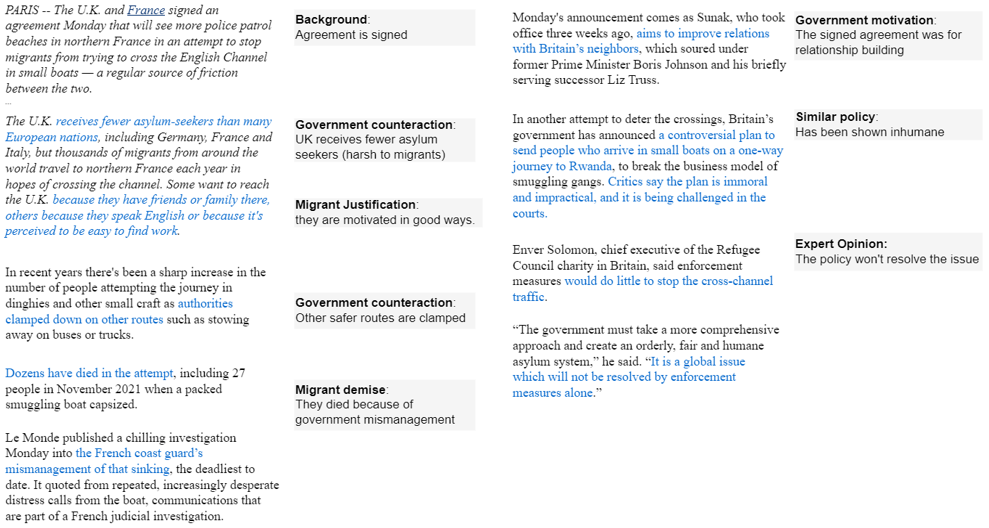
\includegraphics[width=\textwidth]{img/genco-motivation-left}
    \caption{The Subframe-level Dissection of the News Article from a Left-wing News Agency.}
    \label{fig:genco-motivation-left}
\end{figure}

\begin{figure}[ht!]
    \centering
    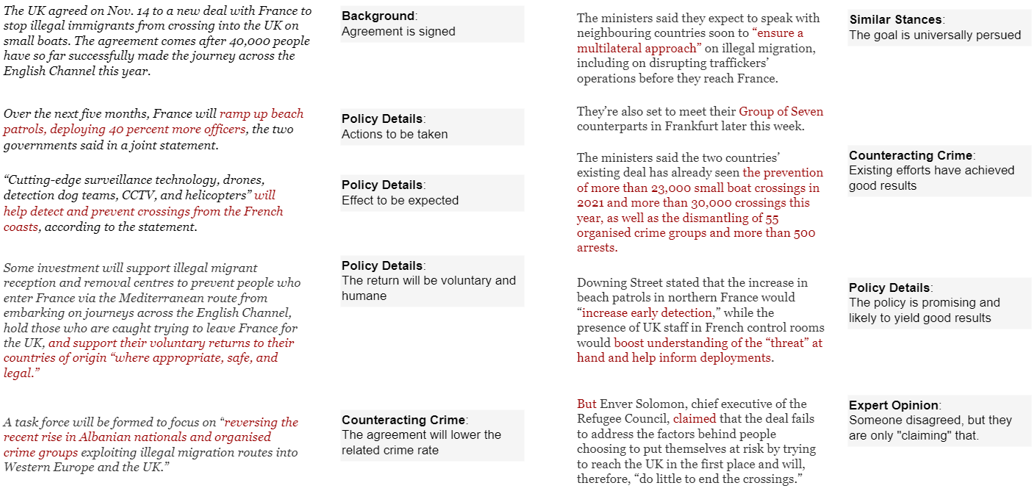
\includegraphics[width=\textwidth]{img/genco-motivation-right}
    \caption{The Subframe-level Dissection of the News Article from a Right-wing News Agency.}
    \label{fig:genco-motivation-right}
\end{figure}

This discrepancy in the news article structures motivates us to hypothesize that the article structure reflects the writer's political stance, and this preference in the article structure, as well as subframe choices, can be modeled by a generative language model. In the next section, we elaborate on our \texttt{GenCo} details and explain how it achieves this goal.

\subsection{GenCo Details}
\label{genco-details}
The architecture of \texttt{GenCo} is shown in \reffig{fig:genco}. The framework starts with an input configuration vector, where the user gets to specify different dimensions of framing, such as political stances and emotional intensity. The vector is then input to a controllable generator which is a generative language model such as \texttt{T5}, \texttt{BART}, and \texttt{GPT}. Existing Information Extraction tools are then applied to extract the event structure of the generated news. We follow \cite{roy-goldwasser-2020-weakly} to extract the subframes and leverage AMR graphs (\eg, \reffig{fig:empirical-amr-left} and \reffig{fig:empirical-amr-right}) with \texttt{amrlib}\footnote{\url{https://github.com/bjascob/amrlib}} to construct article event graphs. Two levels of event graphs are involved: 1) the inter-subframe graphs which capture the coarse-grained semantics such as paragraphs, and 2) the intra-subframe graphs which capture the fine-grained semantics such as sentences. The generator then generates an event graph which is compared to event graphs sampled from corresponding news pools from the dataset for contrastive learning with a classifier. The generator and the classifier are collectively trained and mutually enhancing each other.

\begin{figure}[ht]
    \centering
    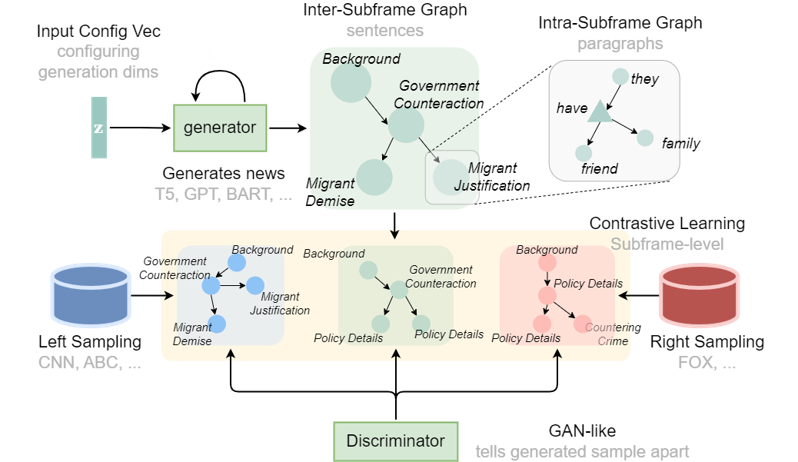
\includegraphics[width=\textwidth]{img/genco}
    \caption{The Architecture of \texttt{GenCo}.}
    \label{fig:genco}
\end{figure}

